\documentclass{article}
\usepackage{listings}
\usepackage{mathrsfs}
\usepackage[utf8]{inputenc}
\usepackage{amssymb}
\usepackage{lipsum}
\usepackage{amsmath}
\usepackage{fancyhdr}
\usepackage{geometry}
\usepackage{scrextend}
\usepackage[english,german]{babel}
\usepackage{titling}
\setlength{\droptitle}{-3cm}
\usepackage{tikz}
\usepackage{algorithm,algpseudocode}
\usepackage[doublespacing]{setspace}
\usetikzlibrary{datavisualization}
\usetikzlibrary{datavisualization.formats.functions}
\usepackage{polynom}
\usepackage{amsmath}
\usepackage{gauss}
\usepackage{tkz-euclide}
\usetikzlibrary{datavisualization}
\usetikzlibrary{datavisualization.formats.functions}
\author{
Alexander Mattick Kennung: qi69dube\\
Kapitel 1
}
\usepackage{import}
\date{\today}
\geometry{a4paper, margin=2cm}
\usepackage{stackengine}
\parskip 1em
\newcommand\stackequal[2]{%
  \mathrel{\stackunder[2pt]{\stackon[4pt]{=}{$\scriptscriptstyle#1$}}{%
  $\scriptscriptstyle#2$}}
 }
\makeatletter
\renewcommand*\env@matrix[1][*\c@MaxMatrixCols c]{%
  \hskip -\arraycolsep
  \let\@ifnextchar\new@ifnextchar
  \array{#1}}
\makeatother
\lstset{
  language=haskell,
}
\lstnewenvironment{code}{\lstset{language=Haskell,basicstyle=\small}}{}
\usepackage{enumitem}
\setlist{nosep}
\usepackage{titlesec}

\titlespacing*{\subsection}{0pt}{2pt}{3pt}
\titlespacing*{\section}{0pt}{0pt}{5pt}
\titlespacing*{\subsubsection}{0pt}{1pt}{2pt}
\title{Vorlesung 4}


\begin{document}
	\maketitle
	\[\bar x\sim Geo^0(p)\]
	\[X:(\Omega, \mathscr{A})\to (\Omega',\mathscr{A}')\]
	1.\\
	\[X:(\Omega, \mathscr{A})\to(\Omega',\mathscr{A}')\]
	Gegeben sei ein W-Modell $(\Omega,\mathscr{A},P)$\\
	Wie kann man aus $(\Omega',\mathscr{A}')$ zu einem W-Modell (mit einem P) ergänzen.\\
	\[A'\in\mathscr{A}': P^X(A')= P(X^{-1}(A')) = P(X\in A')\]
	Also man mapped die A' wieder zurück auf die dazugehörigen A im Urbild (bem.: $X\in A'=\{\omega\in\Omega| X(\omega)\in A\}$)\\
	$(\Omega',\mathcal{A}',P^x)$ ist das Bildmodell von $(\Omega,\mathcal{A},P)$ unter abbildung X.\\
	2.\\
	Unter welchen Vorraussetzungen ist eine Approximation der Binomialverteilung durch die Poisson-.Verteilung sinnvoll:\\
	Viele Messwerte und kleine Wahrscheinlichkeiten\\
	Sei $S_n$ eine Folge von binom. Zufallsvariablen mit Parameter $n\in\mathbb{N}$ und $p_n<<1$ und $\mathbb{E}(S_n) = n\cdot p_n\to \lambda >0$ und $\lim\limits_{n\to\infty} np_n$ (weil man $\lambda =np_n$ setzen möchte) für $n\to\infty$, dann folgt\\
	$P(S_n=k)= B(n,p_n,k) \to \frac{\lambda^k}{k!} e^{-\lambda} = P_\lambda(k)$\\
	\begin{align}\lim_{n\to\infty}P(S_n=k) & = \lim_{n\to\infty}\frac{n!}{k!\,(n-k)!}p^{k}\left(1-p\right)^{n-k}\\
	\text{subst: }p=\frac{\lambda}{n}\implies& =\lim_{n\to\infty}\frac{n!}{k!\,(n-k)!}\left(\frac{\lambda}{n}\right)^{k}\left(1-\frac{\lambda}{n}\right)^{n-k}\\
	 & =\lim_{n\to\infty}\left(\frac{\lambda^{k}}{k!}\right)\left(\frac{n(n-1)(n-2)\cdots(n-k+1)}{n^{k}}\right)\left(1-\frac{\lambda}{n}\right)^{n}\left(1-\frac{\lambda}{n}\right)^{-k}\\
	 & =\frac{\lambda^{k}}{k!}\cdot\lim_{n\to\infty}\underbrace{\left(\frac{n}{n}\cdot\frac{n-1}{n}\cdot\frac{n-2}{n}\cdots\frac{n-k+1}{n}\right)}_{\to1}\underbrace{\left(1-\frac{\lambda}{n}\right)^{n}}_{\to e^{-\lambda}}\underbrace{\left(1-\frac{\lambda}{n}\right)^{-k}}_{\to1}\\
	 & =\frac{\lambda^{k}\mathrm{e}^{-\lambda}}{k!}.
	 \end{align}
	Man kann hieran sehen, dass wenn n sehr groß ist, oder p sehr klein (weil p als $\frac{\lambda}{n}$ dargestellt wird) ist.\\
	3. Aussage des Zentralen Grenzwertsatzes:\\
	Wenn man sehr viele kleine \textbf{unabhängige} Zufallseffekte $n\to\infty$ und kleine Wahrscheinlichkeiten hat $p<<1$ dann kann eine Verteilung als eine Normalverteilung modelliert werden, solange keine einzelne Variable einen dominanten einfluss auf die Varianz besitzt.\\
	Beweis: n i.i.d Zufallsvariablen $X_1,X_2,\dots$: Erwartungswert $\mu$ und std $\sigma$.\\
	$S_n = X_1+X_2+\dots+X_n$ Der Erwartungswert ist $n\mu$ und Var $n\sigma^2$. Standardisieren:\\
	$Z_n = \frac{S_n-n\mu}{\sigma\sqrt{n}}$.\\
	Der zentrale Grenzwertsatz besagt, dass $Z_n$ für $n\to\infty$ zur standardnormalverteilung punktweise konvergiert $\mathcal{N}(0,1)$\\
	z.B.: Sein Bino(n,p) mit großem n und kleinem p, dann gilt:\\
	$F^{S_n} (x) = \Phi(\frac{x-a}{\sigma})$ mit a dem Erwartungswert $\mathbb{E}(S_n)=np$ und $\sigma = \sqrt{np(p-1)}$ weil man n mal das geometrischen Mittel der Wahrscheinlichkeiten hat (geo weil das verhältnisse darstellt)\\
	4.\\
	Negative Bino $nb^+(r, p, k) = \binom{k-1}{r-1} p^r (1-p)^{k-r}$
	oder  $nb^0(r, p, k) = \binom{k+r-1}{r-1} p^r (1-p)^{k}$\\
	(also gleich bis auf substitution).\\
	Namensbegründung: $\binom{n}{k} = \binom{n}{n-k} = \frac{(k+r-1)_k}{k!}$
	$$(k+r-1)_k = (r+k-1)(k+r-2)\dots (r+k-k) = [-(-r-k+1)][-(-r-k+2)]\dots [-(-r)] = (-1)^k(-r)^k$$
	also: \\
	$$\binom{n}{k} = \binom{n}{n-k} = \frac{(k+r-1)_k}{k!} =\underbrace{ |\binom{-r}{k}|}_{negative Binomial} = \frac{(r)_k}{k!}$$
	Kurzes wort zu zufallsvariablen\\
	$X$ gegeben und $Y=g(X)$ allgemeiner Fall.\\
	$$P^Y(Y\leq y) = \underbrace{P^Y(g(x)\leq y)}_{falls\ g\ bijektiv} = P(X\leq g^{-1}(y))$$
	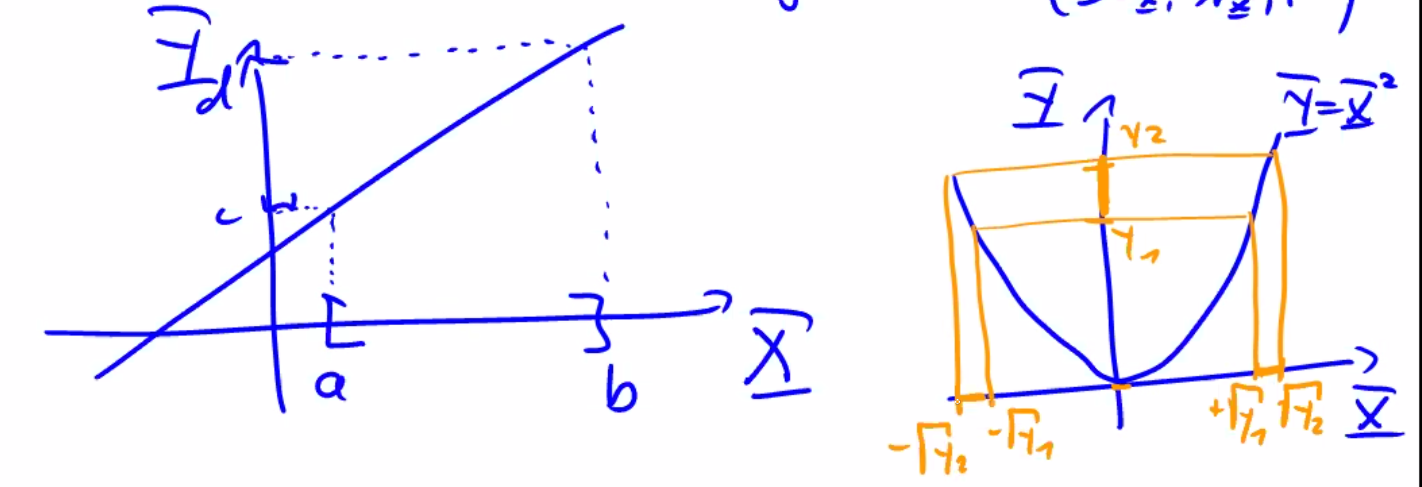
\includegraphics[width=256px]{Zufallsvar.png}\\
	Also falls g nicht bijektiv ist, dann muss man halt stückweise vorgehen (und aufpassen)\\
	Mit affinlinearen abbildungen von ZV $Y=a+bX$
	\[F^Y (y) = F^X(\frac{y-a}{b})\]
	daraus folgt unmittelbar (durc ableiten)
	\[f^Y(y)= \frac{1}{b} f^X(\frac{y-a}{b})\]
\end{document}